% Clase del documento, no tocar, si lo tocas explota el espacio-tiempo y se te

% cae el pito.
\documentclass{article}

%%%%%%%%%%%%%%%%%%%SECCIÓN INCLUSIÓN DE PAQUETES %%%%%%%%%%%%%%%%%%%%%%%%%%%%%%
% Carga el paquete español y permite que los números de página en números 
% romanos sean minúsculas. Técnicamente esto es una falta de ortografía en
% españoles. SI quieres que sean mayúsculas, quita lo de "es-lcroman". 
\usepackage[spanish, es-tabla, es-lcroman]{babel}
% El símbolo del euro viene aparte, señora. Este paquete permite poner el
% símbolo del euro como \euro o formatear como un objeto un número y que ponga
% al final el símbolo haciendo \EUR{numero} por ejemplo \EUR{9,99} pondría
% un precio en euros.
\usepackage{eurosym} 
% este paquete nos permite que las imágenes sean del un tamaño referido al
% ancho de la página.
\usepackage{graphicx}
% nos permite insertar las figures con el especificador H, que hace que se
% inserten donde están puestas y no donde a Latex le salel latexNabo.
\usepackage{float} 
% Paquete que habilita las referencias cruzadas. 
\usepackage{hyperref}
% Permite poner pies y encabezados personalizados
\usepackage{fancyhdr}
 %permite referenciar la última página (para lo de pág. tal de total)
\usepackage{lastpage}
%%%%%%%%%%%%%%%%%%%% FIN SECCIÓN %%%%%%%%%%%%%%%%%%%%%%%%%%%%%%%%%%%%%%%%%%%%%%

% Esto hace que los enlaces a webs (\href{url}{texto} salgan en azul.
% También impide que salga un repugnante recuadro rojo alrededor de cada
% referencia cruzada que incluyas en el documento.
\hypersetup{
    colorlinks=true,
    linkcolor=black,
    filecolor=magenta,      
    urlcolor=blue,
}
% Permite que en las ecuaciones escribas un punto y salga un punto (no lo
% interprete como un decimal en español, es decir, una coma)
\decimalpoint

%%%%%%%%%%%%%%%%%SECCIÓN VARIABLES %%%%%%%%%%%%%%%%%%%%%%%%%%%%%%%%%%%%%%%%%%%%
% Podemos definir variables para usar a lo largo del texto
% Así podemos cambiarlas aquí sin tener que repetir texto.
\def \autor{Pablo Francisco Fernández Fernández}
\def \titulo{Ejemplo de documento en \LaTeX}
\def \organizacion{Universidad de Vigo}
%%%%%%%%%FIN SECCIÓN%%%%%%%%%%%%%%%%%%%%%%%%%%%%%%%%%%%%%%%%%%%%%%%%%%%%%%%%%%%

% Esta orden especifica que cuando se cree la portada se use este título.
% Además, con Huge utilizamos la macro de tipo de letra más grande que hay 
% disponible.
\title{\textbf{\Huge{\titulo}}}
% Aquí lo mismo, pero con el autor, Large es otra macro de tamaño, y LARGE otra 
\author{\LARGE{\autor}\\ \\ \Large{\organizacion}}

%%%%%%%%%%%%%%%%%%%%%%%%%%%%%%INICIO DEL DOCUMENTO%%%%%%%%%%%%%%%%%%%%%%%%%%%%%
% La totalidad del texto que se renderizará en PDF en tu documento debe estar
% entre begin document y end document.
\begin{document}
% Elimina la numeración de página hasta que se diga lo contrario.
\pagenumbering{gobble}
% Pone el título, el autor y la fecha.
\maketitle

% Aquí creamos una figura para poner el logo de algo (he elegido la UVigo), 
% más en cuanto a figuras más adelante.
\begin{figure}[H]
% Lo centramos
\center
\includegraphics[width=.5\linewidth]{./img/escudouvigo}
\end{figure}
\newpage
% En esta página puedes poner agradecimientos o prefacios que no tendrán pie ni
% encabezado de página y que no afectarán a la numeración, si no quieres poner
% nada, elimina esta línea y uno de los newpages
\textbf{[Esta página ha sido dejada en blanco a propósito por el editor]}
\newpage
%Vamos a poner agradecimientos
\begin{flushright}
\textit{Agradezco a mi psicóloga que me ha entrenado para no querer tirarme por
la ventana al estar utilizando esta herramienta para psicópatas del demonio.\\
También a Stack Overflow que me he permitido hacer esto }
\end{flushright}
\newpage % salto de página

%%%%%%%%%%%%%%%%% CABECERA Y PIE DE PÁGINA SECCIÓN ÍNDICE%%%%%%%%%%%%%%%%%%%%%
\pagestyle{fancy}
\fancyhf{}
\rhead{\autor}
\lhead{\titulo}
\rfoot{pág. \thepage{} de \pageref{startSectionContent}} 
\renewcommand{\footrulewidth}{0.5pt}
\pagenumbering{roman} %decimos que se numeren las páginas en romano
%%%%%%%%%%%%%%%%%FIN
\tableofcontents %crea el índice el índice empieza siempre en página nueva

% se pueden añadir saltos de página extra con \newpage
\newpage

% cambia el nombre del índice de ilustraciones
\renewcommand{\listfigurename}{Índice de ilustraciones}
%inserta el índice de ilustraciones
\listoffigures 
\newpage

%tambia el nombre del índice de tablas
\renewcommand{\listtablename}{Índice de tablas}

%inserta el índice de tablas
\listoftables

% Esta orden (label) inserta etiquetas invisibles en el texto, al ponerla justo
% antes del salto de página del último índice de la sección, me permite
% referenciar este punto, así es como consigo que salga "Pág. i de iiii".
\label{startSectionContent}

\newpage

%%%%%%%%%%%%%%%%% CABECERA Y PIE DE PÁGINA SECCIÓN CUERPO%%%%%%%%%%%%%%%%%%%%%%
\pagestyle{fancy}
\fancyhf{}
\rhead{\autor}
\lhead{\titulo}
\rfoot{pág. \thepage{} de \pageref{LastPage}}
\renewcommand{\footrulewidth}{0.5pt}
%%%%%%%%%%%%%%%%%FIN SECCIÓN%%%%%%%%%%%%%%%%%%%%%%%%%%%%%%%%%%%%%%%%%%%%%%%%%%%

\section{Primera sección}
% A partir de ahí numeración normal
\pagenumbering{arabic}

% párrafo con texto en distintos formatos, textit es itálita, textbf es 
% negrita, se pueden combinar. texttt es monoespaciada, la uso luego
% Como puedes ver, aunque hay saltos de línea, no son párrafos distintos.
% Para que sean párrafos distintos tiene que haber una línea en blanco
% entre ellos.
Estoy escribiendo un artículo que mola mazo sobre cosas interesantes.
Cosas tan interesantes que ahora tienen que ir en \textbf{negrita} y en
\textit{cursiva}. Algunas cosas, de hecho, tienen que ir en
\textbf{\textit{negrita y cursiva.}}

%%% Ejemplo de lista
A veces tengo que poner listas.
Esta es una lista de cosas que me gusta poner en las tostadas.
% Este tipo de listas no son numeradas. Son listas de puntitos.
\begin{itemize}
    % Un item es una fila de la lista, un punto, en este caso.
    \item Mantequilla
    % si quieres subniveles, creas una lista dentro de esta.
    % Ojo, cuidado, tiene que haver un item antes, como aquí que está
    % el item mantequilla.
    \begin{itemize}
        \item A veces es margarina
        \begin{itemize}
            \item A veces es de aceite de olive
            \item Otras es de aceite de girasol
        \end{itemize}
        \item Nunca manteca, pero quizá esté bueno.
    \end{itemize}
    \item Mermelada
    \item Nocilla
    \item Azúcar
\end{itemize}


Los elementos más importantes de la política del siglo XX son... no sé, no sé
de eso, estoy sólo rellenando texto. \textbf{Me gusta la letras en negrita}.
Ahora voy a poner una fórmula matemática, porque me da la gana.
% Fórmula matemática en su propio párrafo, utilizando dos signos de dolar.
$$
G\frac{m_1 m_2}{d^2}
$$

Si en este párrafo quisiéramos poner una ecuación o números al estilo 
matemático, lo haremos con único signo de dolar $a^2+b^2+c$. 
Además, podemos poner símbolos monetarios gracias a algunos paquetes especiales
(ver en donde se incluyen los paquetes). \EUR{10.000.000} Para poner un dolar
simplemente pones \$, por ejemplo: Ayer me encontré 50 \$ en un bolsillo.

\subsection{Sección de segundo orden}

Como podemos ver, una subsección se define fácilmente, con la orden
\texttt{\textbackslash subsection}, también existe \texttt{\textbackslash
subsubsection}. A partir de ahí, si quieres títulos de un nivel más profundo,
hay que usar otras órdenes.
\subsubsection{Tercer nivel en la jerarquía}
Si quieres más información sobre ćomo hacer esto, puedes visitar
\href{https://ctan.org/pkg/titlesec}{este enlace}.
Pero es una movida \textbf{de cojones}.
\section{Segunda sección}
Aquí yo tenía un párrafo sobre cuando uśabamos la clase report, pero lo cambié
en esta versión a la clase article, así que no ha lugar. Si quieres usar la 
otra clase, míralo allí. No lo recomiendo.
% Los bloques verbatim son bloques donde el texto se inlcuye sin tomar en 
% cuenta comandos de latex y en letras monoespaciada.
% Se suelen usar para introducir código.
\begin{verbatim} 
int main(void){
    std::vector<int> v{1,2,3,4,5};
    for(auto i : v){
        std::cout << i << std::endl;
    }
    return EXIT_SUCCESS;
}
\end{verbatim}
Aquí vamos a poner otro párrafo, que no sé si se va a cargar. Hola. ¿Funciona
esto? Sí, parece ser que sí funciona. Pues ahora vamos a poner una lista de
cosas con numeración. Gracias a que hemos cargado el paquete babel español,
podemos utilizar $<<$ y $>>$ para poner comillas latinas. Por ejemplo:

% Dos barras invrtidas (\\) fuerzan un salto de línea.
<<El día que la mierda tenga algún valor, los pobres nacerán sin culo>> \\
--Gabriel García Mázquez

% Lista con enumeración (Nótese que entre llaves pone enumerate)
\begin{enumerate}
\item Primer elemento
    \item segundo elemento
        \begin{enumerate} %sublista
            \item cosas
                \begin{enumerate}
                    \item bla
                \end{enumerate}
            \item otras cosas
        \end{enumerate}
    \item tercer elemento
\end{enumerate}

Para poner una imagen hay que poner \texttt{\textbackslash
includegraphics\{<ruta a la imagen, puede ser relativa>\}}
Con el la línea \texttt{\textbackslash graphicspath\{ruta\}}
puedes decirle a latex que las imágenes están en esa ruta y así sólo tienes
que poner el nombre. Por ejemplo, si tenemos este árbol de directorios:

\begin{verbatim}
.
|-- briefing.pdf
|-- briefing.tex
|-- img
    `-- gatito.jpg
\end{verbatim}

Pues la orden que deberíamos poner es \texttt{\textbackslash
graphicspath\{img\}}. Y entonces sólo tendríamos que escribir el nombre de las
imágenes (sin extensión).

% Así se incluye una imagen. Predeterminadamente, se incluye a su tamaño 
% original
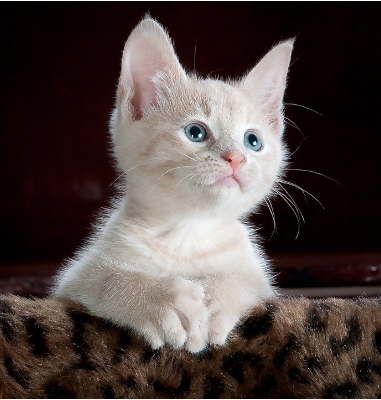
\includegraphics{./img/gatito}
Con la opción scale podemos hacerla más pequela -o más grande-.
Pero así sólo estamos poniendo la imagen en el texto, esto quería bien para un
párrafo como de revista donde estás hablando de gatitos, en este caso, y
empiezas a decir cosas sobre ellos.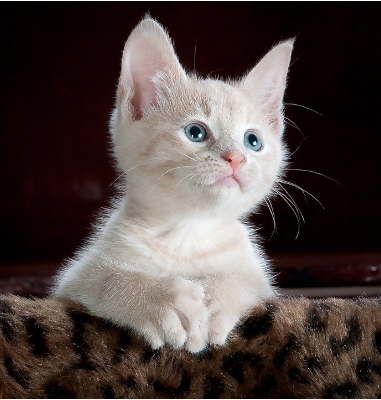
\includegraphics[scale=0.2]{./img/gatito}.
Mira qué monos los gatitos, cómo me gustan los gatitos, ay los gatitos qué
majetones. Lo que hay que hacer para que se inserte como una figura es utilizar
un bloque de figura.

% [H] inserta aquí, t al inicio de la página, b al final... muchas cosas
% Usa "H", me lo agradecerás, si no Latex decice dónde poner las cosas según su
% criterio. Para usar "H" hay que incluir el paquete float
% (ver sección donde incluyo los pauqetes)
\begin{figure}[H]
    % Centra la imagen
    \centering 
    % Con width=1.0\hsize hacemos que la imagen sea tan ancha como el párrafo,
    % yo lo recomiendo para que las cosas queden alineadas, salvo que por x
    % motivo quieras una imagen más pequeña, entonces usa scale y ve jugando.
    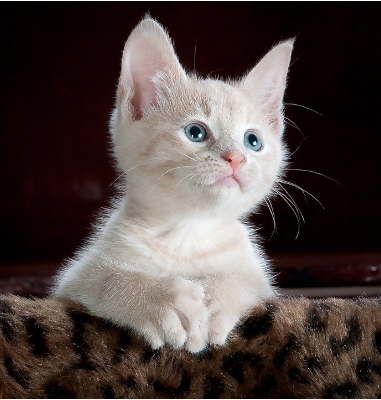
\includegraphics[width=1.0\hsize]{./img/gatito}
    % Título de la figura que se ve
    \caption{Un gato naranja}
    % Etiqueta interna, se usa para referencias la imagen. Esta orden debe ir
    % siempre después de la caption. Cada tipo de figura tiene su formato de 
    % label, por ejemplo las figuras son fig: y las tablas tab:, respétalo o 
    % LaTeX no podrá encontrarlas para los índices.
    \label{fig:gatitoNaranja} 
\end{figure}

Al insertar un párrafo aquí podemos ver cómo se organizan las imágenes, de tal
modo que se insertan en la página necesaria. Las figuras no se dividen a sí
mismas entre páginas, según tengo entendido, así que no hay que preocuparse
de eso.

\begin{figure}[H]
    %centra la imagen (por si no quedaba clarinete)
    \centering
    % El número antes de hsize es un multiplicador, por ejemplo, podemos hacer
    % que ocupe un tercio de ancho
    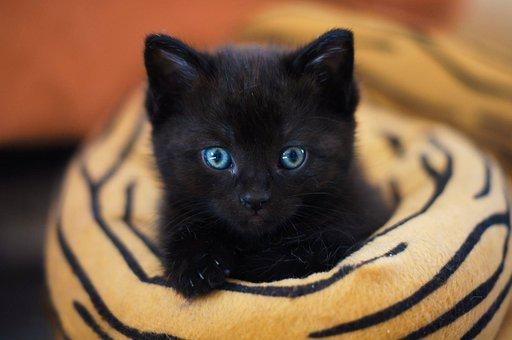
\includegraphics[width=0.3333\hsize]{./img/gatitoNegro}
    \caption{Un gato negro} %caption que se ve
    \label{fig:gatitoNegro} %nombre interno para referenciar luego
\end{figure}

Si ahora quieres referenciar una figura en un párrafo en \LaTeX puedes poner
\texttt{ \textbackslash ref\{nombre de la referencia\}}.
Por ejemplo: como podemos ver en la ilustración \ref{fig:gatitoNegro}
\nameref{fig:gatitoNegro}. Como sorprendentemente no me he arrancado ya la piel
a tiras con esta herramientas para masoquistas, vamos a insertar una tabla.
% Esto no sirve para hacer la tabla en sí misma, sino para ponerle captions y
% esas cosas. Es equivalente a \begin{figure} que no inserta una imagen, pero
% nos prepara las cosas para que se comporte como una figura, así podemos
% ponerle título y referenciarla.
\begin{table}[H]
    % Aquí defines la tabla en sí misma, tienes que poner tantas letras como
    % columnas vaya a tener la tabla, y puedes poner líneas verticales entre
    % ellas escribiendo este símbolo entre las letras. Estas letras son los
    % especificadores de alineación. Si pones l, la columna se alinea a la
    % izquierda, si pones c, al centro, y si pones r, a la derecha.
    \begin{tabular}{|c|r|c|r|}
    % Esta orden genera una línea entre filas de la tabla.
    \hline
    % En las tablas las celdas se separan con & y las filas con \\
    % Puede haber celdas vacías, pero todas las filas deben tener las mismas
    % celdas.
    Concepto & Precio Unitario & Cantidad & Subtotal\\ \hline
    Placa base & \EUR{89.99} & 1 & \EUR{89.99}\\ \hline
    Memoria RAM 8GB DDR4 3200 MHz & \EUR{40.44} & 4 & \EUR{161.76} \\ \hline
    % Aquí podemos ver que hemos puedo celdas vacías. (dos & seguidos)
    \textbf{Total}&&&\textbf{\EUR{251.75}} \\ \hline
\end{tabular}
    % De nuevo, el título que se ve
    \caption{Gastos de la reparación}
    % La referencia interna. 
    \label{tab:gastos}
\end{table}

De nuevo, podemos referenciar el número de la tabla con \ref{tab:gastos} y su
títulos con \nameref{tab:gastos}. Nota del tío Paco: a veces salen signos de
interrogación, no te preocupes, \LaTeX a veces necesita dos compilaciones para 
crear la base de datos de referencias.

Creo que ya estás listo para usar \LaTeX. Me gusta \textit{whisky} que alguna
gente escribe \textit{whiskey}. También me gusta el bebercio en general, general
capitán, rey del champán. Bla bla bla bla bla. a a a a 

\begin{center}
    \tiny{The End}

    \small{The End}

    \large{The End}

    \Large{The End}

    \LARGE{The End}

    \huge{The End}

    \Huge{The End}
\end{center}

\end{document}
